\documentclass[10pt,a4paper]{amsart}

\usepackage{lmodern}
\linespread{1.1}
\usepackage[utf8]{inputenc}
\usepackage[T1]{fontenc}
\usepackage[icelandic]{babel}

\usepackage{fancyref}
\usepackage[colorlinks=true]{hyperref}
\usepackage{xcolor}

\usepackage{tikz}
\usetikzlibrary{calc}

\author{Gunnar \TH\'or Magn\'usson}
\title[Lengdin \'a hringveginum]{Hver er munurinn á að keyra\\
hringveginn réttsælis eða rangsælis?}

\begin{document}

\maketitle

Á hringveginum er yfirleitt akrein í sitt hvora áttina. Önnur þeirra er nær
miðpunkti landsins en hin, svo lengd hennar ætti að vera styttri en lengd
hinnar. Spurningin er hvort við vitum hversu mikið styttri hún sé og hvort við
getum reiknað það?

Okkur ætti að vera ljóst að við getum svarað þessari spurningu ef við fáum til
þess langa helgi, bensínpening og einhverjar byrgðir af kaffi. Við þurfum
einfaldlega að keyra hringveginn tvisvar, einu sinni réttsælis og einu sinni
rangsælis og lesa af kílómetramælinum hversu löng sitt hvor leiðin var.
Lesendur eru hvattir til að gera það við tækifæri og bera niðurstöður sínar
saman við greiningu okkar hér.

Áður en við leggjum í meiri útreikninga skulum við byrja á því að athuga
einfaldari útgáfu af spurningunni til að fá tilfinningu fyrir hvað gæti verið
rétt: Gerum ráð fyrir að hringvegurinn sé hringur. Við skulum þá segja að
réttsælisvegurinn hafi geislann $r$ og að
rangsælisvegurinn hafi geislann $R$, og vegna þess að umferð á Íslandi keyrir
hægra megin er þá $r < R$. Við skrifum því $R = r + b$, þar sem $b$ er bilið á
milli veganna (sjá mynd~\ref{fig1}).
\begin{figure}[h!]
	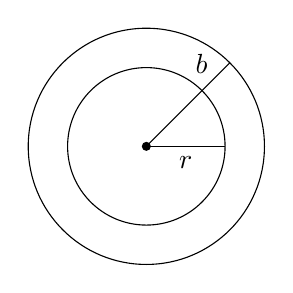
\begin{tikzpicture}
		\draw (0,0) circle [radius=1.5];
		\draw (0,0) circle [radius=1];
		\draw (0,0) -- (1,0);
		\draw (0,0) -- (1.06,1.06);
		\node[below] at (0.5,0) {$r$};
		\node[above left] at (0.9,0.8) {$b$};
		\draw[fill=black] (0,0) circle [radius=0.05];
	\end{tikzpicture}
	\caption{Hringir með sömu miðju og geisla $r$ og $r+b$.}
	\label{fig1}
\end{figure}
Ummál hrings með geisla $r$ er $2\pi r$, svo að munurinn á
þessum vegalengdum er
$$
2\pi (r + b) - 2 \pi r = 2 \pi b.
$$
Nú skulum við skoða upphaflegu spurninguna aftur. Við þurfum eitthvað
stærðfræðilegt líkan af hringveginum, og það virðist eðlilegt að skoða það sem
stærðfræðingar kalla \emph{veg}: Það er samfellt og deildanlegt fall $f : [0,1] \to
\mathbb{R}^2$ sem endar þar sem það byrjar, sem þýðir að $f(1) = f(0)$ (sjá mynd~\ref{fig2}). Við
getum gert ráð fyrir að fallið sem við veljum sé réttsælisvegurinn; í
einfaldari útgáfunni hér að ofan væri þá $f(t) = (r \cos 2\pi t, r \sin 2\pi
t)$. Við ætlum þar að auki að gera ráð fyrir að vegurinn skeri sjálfan sig
ekki, og að hann fari aðeins einn hring í kringum landið.

\begin{figure}[ht]
	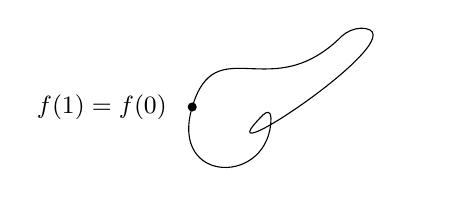
\begin{tikzpicture}
		\draw [rounded corners]
			(0,0) .. controls (0.3,1) and (1,0) ..
			(2,1) .. controls (3,1) and (0,-1) ..
			(1,0) .. controls (1,-1) and (-0.3,-1) .. (0,0)
			;
		\node[left] at (-0.2,0) {\small $f(1) = f(0)$};
		\draw[fill=black] (0,0) circle [radius=0.05];
	\end{tikzpicture}
	\caption{Vegur.}
	\label{fig2}
\end{figure}

Til að búa til rangsælisveginn út frá þessum ætlum við að bjaga réttsælisveginn
aðeins ``út á við'', sem þýðir stærðfræðilega í áttina að normalvigri sínum.
Snertivigurinn $f'(t)$ við veginn táknar stefnu og hraða okkar á tíma $t$.
Normalvigurinn $\nu(t)$ er svo vigurinn sem er hornréttur á $f'(t)$, vinstra
megin við hann, og hefur lengdina $1$. Að þessu loknu er rangsælisvegurinn
okkar þá $g(t) = f(t) + b \nu(t)$, þar sem $b$ er bilið á milli veganna
tveggja (sjá mynd~\ref{fig3}).

\begin{figure}[hb]
	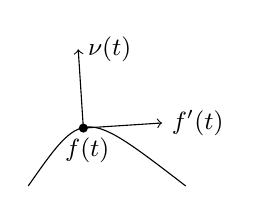
\begin{tikzpicture}
		\draw (-1,0) .. controls (-0.3,1) .. (1,0);
		%\draw (-1,0.25) .. controls (-0.3,1.2) .. (1,0.25);
		\draw[fill=black] (-0.3,0.735) circle [radius=0.05];
		\draw[->] (-0.3,0.735) -- (0.7,0.8);
		% v = (1, 0.065)
		% n = (-0.65, 1)
		% (-0.95, 1.735)
		\draw[->] (-0.3,0.735) -- (-0.365,1.735);
		\node[right] at (0.7,0.8) {\small $f'(t)$};
		\node[right] at (-0.365,1.735) {\small $\nu(t)$};
		\node[below] at (-0.25,0.73) {\small $f(t)$};
	\end{tikzpicture}
	\caption{Snerti- og normalvigrarnir skilgreina rangsælisveginn.}
	\label{fig3}
\end{figure}

Til að reikna lengdina $L(f)$ á vegi $f$ reiknum við heildið
$$
L(f) = \int_0^1 \|f'(t)\| dt,
$$
þar sem $\|f'(t)\|$ er lengd $f'(t)$, sem við þekkjum betur sem hraðann sem við
keyrum á. Þá sjáum við að lengd rangsælisvegsins er
$$
L(g) = \int_0^1 \|g'(t)\| dt
= \int_0^1 \|f'(t) + b \nu'(t)\| dt.
$$
\href{https://en.wikipedia.org/wiki/Frenet%E2%80%93Serret_formulas}{Frenet og Serret} reiknuðu út að $\nu'(t) = - \kappa(t) f'(t)$, þar sem
	$\kappa(t)$ er \href{https://en.wikipedia.org/wiki/Curvature#Plane_curves}{\emph{krappi}} vegsins $f$ í punktinum $t$. Krappinn er mælikvarði á
	hversu mikið vegurinn beygir á hverjum stað; bein lína hefur krappann núll, á
	meðan að hringur hefur alls staðar sama krappann. Með þessari formúlu sjáum við
	að
	$$
	L(g) = \int_0^1 |1 - b\kappa(t)| \|f'(t)\| dt.
	$$
	Til að komast lengra ætlum við að beita stærðfræðilegum brellum. Stærðin
	$\|f'(t)\|$ táknar hraðann sem við keyrum á. Með því að keyra á hraðanum $1$
	í $L(f)$ tíma, sem við hefðum hugsanlega ekki þolinmæði fyrir í
	alvörunni, þá er lengdin á réttsælis hringveginum einfaldlega $L(f) =
	\int_0^{L(f)} dt$. Þá einfaldast hitt heildið og lengdin á rangsælisveginum
	verður
	$$
	L(g) = \int_0^{L(f)} |1 - b\kappa(t)| dt.
	$$
	Ef við getum réttlætt að $b\kappa(t) < 1$ fyrir öll $t$ þá getum við reiknað
	algildið undir heildinu. En eftir smá umhugsun ættum við að geta gert ráð fyrir því:
	Breiddin $b$ er aðeins einhverjir metrar, og því stærri sem krappinn er því
	erfiðara er að taka beygjur eftir veginum. Þar sem fólk má keyra á 90 km/klst
	eftir mestmegninu á hringveginum getum við gert ráð fyrir að krappi hans sé
	frekar lítill, svo við skulum segja að skilyrðinu $b\kappa(t) < 1$ sé fullnægt.
	En þá erum við langt komin, því að mismunurinn á lengd veganna er þá
	$$
	L(g) - L(f)
	= \int_0^{L(f)} b \kappa(t) dt.
	$$
	Nú er \href{https://en.wikipedia.org/wiki/Total_curvature}{merkileg staðreynd} að heildið á krappanum yfir allan veginn er
	einfaldlega $2\pi$, alveg sama hver vegurinn $f$ er, svo lengi sem hann fer
	aðeins einn hring. Svarið við upprunalegu spurningunni er því að mismunurinn á
	lengdunum milli veganna er
	$$
	L(g) - L(f)
	= 2 \pi b,
	$$
	þar sem $b$ er bilið á milli þeirra, alveg eins og í einfölduðu útgáfunni með hringjunum í upphafi.
	Það sem er sérstaklega merkilegt við þessa útkomu er að hún er algjörlega óháð hversu langur vegurinn er, það eina sem skiptir máli er bilið $b$ á milli rétt- og rangsælishluta hans.
	Við getum svarað spurningu um allan hringveginn með því að fara út á næstu götu og mæla bilið milli akreina þar.

	Að þessu loknu er ágætt að skoða aftur þá hluti sem við höfum gert ráð fyrir
	til að komast hingað. Við gáfum okkur að hringvegurinn hefði ekki stóran krappa
	miðað við bilið á milli veganna tveggja, sem hlýtur að teljast raunhæft ef það
	á að vera hægt að keyra veginn á skynsamlegum hraða. Við gáfum okkur einnig að
	bilið $b$ á milli veganna væri alls staðar eins til að geta reiknað lokaheildið. Þetta er
	ekki satt í alvörunni, svo líkan okkar gefur ekki alveg rétt svar. Hins vegar
	getum við notað þetta líkan til að fá neðri og efri mörk $2\pi b \leq L \leq
	2\pi B$, þar sem $b$ og $B$ eru minnstu og stærstu bilin milli veganna og $L$
	er hið raunverulega svar.

	Í lokin getum við ekki stillt okkur um að minnast á að þessir útreikningar
	útskýra af hverju rásmerkingar á hlaupabrautum eru á mismunandi stöðum. Ef
	lesendur hafa horft á hlaup á Ólympíuleiknum hafa þeir kannski séð að rásmerkin
	á ytri hlaupabrautum eru ekki á sama stað og merkin á þeim innri. Á hlaupabraut
	þar sem innsta brautin er 400 metrar er næst-innsta brautin 407.7 metra löng,
	þar næsta braut er 415.3 metrar, og sú þriðja 423 metrar. Mismunurinn hér er
	alltaf sá sami, eða um 7.7 metrar. Hver braut er 1.22 metra breið, og $2\pi *
	1.22 \cong 7.665$, svo rásmerking ytri brautar þarf að vera sirka 7.66 metrum
	framar merkingu innri brautar til að hlauparar á þeim báðum hlaupi sömu
	vegalengd.

	\end{document}
